%% ---------------------------------------------------------------------------
%% intro.tex
%%
%% Introduction
%%
%% $Id: intro.tex 1477 2010-07-28 21:34:43Z palvarado $
%% ---------------------------------------------------------------------------

\chapter{Introducción}
\label{chp:intro}

\section{Entorno del proyecto}

El control automático de sistemas es una rama de la ingeniería que se dedica al diseño y análisis de sistemas de control que de manera automática buscan satisfacer criterios de optimalidad preestablecidos. Estos sistemas se utilizan en aplicaciones que abarcan desde el control de procesos industriales hasta el control de sistemas de navegación en vehículos autónomos, donde para lograr un control automático efectivo, se emplean técnicas y algoritmos, como el control proporcional-integral-derivativo (PID), el control adaptativo, el control moderno y otros \textcolor{SkyBlue}{ControlModerno}. La implementación de estos sistemas requiere del uso de hardware y software especializados, así como del conocimiento en áreas de la electrónica, informática y actualmente, la aplicación de la inteligencia artificial (IA) \textcolor{SkyBlue}{Kuo}.

El campo de aplicación de la IA está en constante crecimiento, impulsado por la necesidad de automatizar procesos y mejorar la eficiencia en diversas industrias. La IA se utiliza en sistemas de control para incrementar la precisión y velocidad de respuesta, apoyando así la toma de decisiones en tiempo real \textcolor{SkyBlue}{IntroSistemasControl} \textcolor{SkyBlue}{SistemaAlmidon}. Algunas de las aplicaciones más comunes incluyen la robótica, el control de procesos industriales, la domótica y la automatización de vehículos \textcolor{SkyBlue}{MarketResearch}. De acuerdo con un informe de Allied Market Research \textcolor{SkyBlue}{MarketResearch}, se espera que el mercado global de sistemas controlados mediante IA alcance los $\$ 30.8$ mil millones para el año 2026, con una tasa de crecimiento anual compuesta del $33.7\%$ desde 2019 hasta 2026. Se espera que la creciente demanda de soluciones de automatización, la evolución de esta tecnología y la creciente inversión en investigación y desarrollo impulsen aún más el crecimiento de este mercado en los próximos años \textcolor{SkyBlue}{MarketResearch}.

El fuerte aumento en la introducción del uso de IA en diversos ámbitos del mercado mundial, obliga a las universidades, a mantenerse activas en la propuesta y mejora de aplicaciones para la IA y su correspondiente divulgación. Esto se observa en la tendencia de investigaciones de las universidades líderes en tecnología a nivel mundial, como el Massachusetts Institute of Technology (MIT), la Universidad de Stanford, la Universidad de Oxford, entre otras \textcolor{SkyBlue}{UniversidadesIA}. Los experimentos que se realizan incluyen el desarrollo de algoritmos de aprendizaje automático para analizar grandes conjuntos de datos y descubrir patrones y tendencias, la aplicación de técnicas para resolver problemas en campos tan diversos como la medicina, la ingeniería, las ciencias sociales, además de la investigación en el uso de estas herramientas para mejorar la eficacia de los sistemas educativos \textcolor{SkyBlue}{MachineLearning}. Estos proyectos no solo están ayudando a los estudiantes a adquirir habilidades valiosas y a estar mejor preparados para los desafíos del mundo laboral, sino que también están generando nuevas oportunidades de investigación y desarrollo en áreas clave. Algunos ejemplos son la utilización de redes neuronales para la predicción del rendimiento académico, detección de enfermedades, identificación de aves, reconocimiento de emociones, entre otros \textcolor{SkyBlue}{MachineLearning}.

Alineado con lo anterior, el SIPLab de la Escuela de Ingeniería Electrónica del Instituto Tecnológico de Costa Rica, busca desarrollar soluciones a problemas regionales y nacionales en el campo mencionado anteriormente, esto mediante proyectos de procesamiento de señales donde se integre el aprendizaje automático y sus aplicaciones, permitiendo que estudiantes y profesores incursionen en el tema de la inteligencia artificial y la apliquen en sus actividades academicas \textcolor{SkyBlue}{SIPLab}. 



\section{Planteamiento del problema}

\subsection{Generalidades}

En la actualidad, el incremento en la complejidad de las plantas de control y su variedad de componentes dificulta el diseño del controlador y su optimización. Una solución prometedora para este problema es la aplicación de técnicas de aprendizaje automático, específicamente el aprendizaje reforzado (RL), el cual permite que un sistema aprenda de su experiencia y adapte su comportamiento para lograr una tarea específica, esto gracias a un diseño eficiente en la toma de muestras de información, su interpretación y modelado respectivo. Este RL presenta una variedad considerable de métodos que posibilitan su clasificación en distintas categorías, siendo las principales el aprendizaje reforzado basado en un modelo y el aprendizaje reforzado sin modelo \textcolor{SkyBlue}{AprendRefor} \textcolor{SkyBlue}{DataScience}.

El RL como tal requiere tener un panorama claro del objetivo a cumplir para la correcta elección de métodos de aprendizaje congruentes y así, lograr optimizar el comportamiento de un agente en el entorno, donde los principales tipos de métodos de RL son: el RL basado en modelo (\textit{Model-based RL}, MBRL), RL sin modelo (\textit{Model-free RL}, MFRL) y el RL profundo (\textit{Deep RL}). El MBRL usa un modelo del entorno mediante el cual se aplican iteraciones de políticas o valores para el proceso, lo cual representa un enfoque más dirigido a la prueba y error en el entrenamiento del modelo con programación dinámica.  El MFRL efectua una relación más directa con el ambiente a controlar, únicamente basándose en experiencias obtenidas por contextualización como el caso de la aplicación de la función $Q$ con el \textit{Q-learning} o SARSA. El Deep RL combina los métodos anteriores con redes neuronales profundas, lo que le permite representar y procesar datos más complejos (alta dimensión) y mejorar el rendimiento del agente sin necesidad de extraer características manualmente del entorno \textcolor{SkyBlue}{DataScience}

En términos generales, para realizar un diseño de un controlador con aprendizaje reforzado es necesario el conocimiento en ingeniería en electrónica, en particular el diseño y construcción de sistemas electrónicos, teoría de sistemas, sistemas digitales, sensores y actuadores, de manera que se pueda garantizar la implementación eficiente, precisa y confiable que integre, además, técnicas del aprendizaje automático \textcolor{SkyBlue}{Control} \textcolor{SkyBlue}{BBVA} \textcolor{SkyBlue}{VideoIA}.

Como contexto para este proyecto, se parte del trabajo de Brenes Alfaro \textcolor{SkyBlue}{TesisJorge}, quien propuso un sistema basado en redes neuronales, para emular el comportamiento de una planta de laboratorio, específicamente el Péndulo Amortiguado a Hélice (PAMH), comúnmente utilizado en el Laboratorio de Control Automático de la Escuela de Ingeniería Electrónica del ITCR. Así, se cuenta con una red neuronal que se comporta de manera similar a la versión física de la planta, considerando perturbaciones y otros factores que definen el comportamiento de la planta real \textcolor{SkyBlue}{PAMHinfo}, y que permite entonces ser usada en enfoques libres de modelo para el diseño de controladores, usando técnicas de aprendizaje reforzado, sin arriesgar la integridad de la planta real, y permitiendo su uso en tiempo de simulación acelerado.

En este punto, se cuenta con un modelo del comportamiento de la planta de laboratorio PAMH. Sin embargo, no se ha propuesto aun ningún método de control basado en aprendizaje reforzado \textcolor{SkyBlue}{TesisJorge}, donde los métodos más comunes son basados en modelos y sin modelo. El primero presenta iteraciones con políticas o valores programados dinámicamente, mientras que el segundo se basa en cálculos de optimización con gradiente o libres de él. Además, se denomina el apartado de aprendizaje reforzado profundo (\textit{Deep RL}) como una combinación de los métodos mencionados \textcolor{SkyBlue}{DataScience}.

De esta manera, la problemática planteada desde el punto de vista ingenieril apunta a una premisa enfocada al aprendizaje automático aplicado mediante el RL para el control automático.

\subsection{Síntesis del problema}

Se carece de un sistema de control automático, que por medio de técnicas de aprendizaje reforzado, permita manipular el comportamiento de una planta de control no lineal.



\section{Enfoque de la solución}

Ahora que se conoce la problemática y el entorno de este proyecto que persigue aplicar el aprendizaje automático al control de una planta no lineal, es necesario plantear algunas opciones que permitan resolver dicho problema, las cuales se ven direccionadas a los métodos y algoritmos de aprendizaje existentes.

Así, se proponen tres alternativas que permiten el control de la planta PAMH (Figura \ref{fig:PAMH}) con diferentes frentes de operación de aprendizaje reforzado. Este tipo de aprendizaje en general mantiene una estructura como la mostrada en la Figura \ref{fig:EstructuraAR}.

\begin{figure}[h]
    \centering
    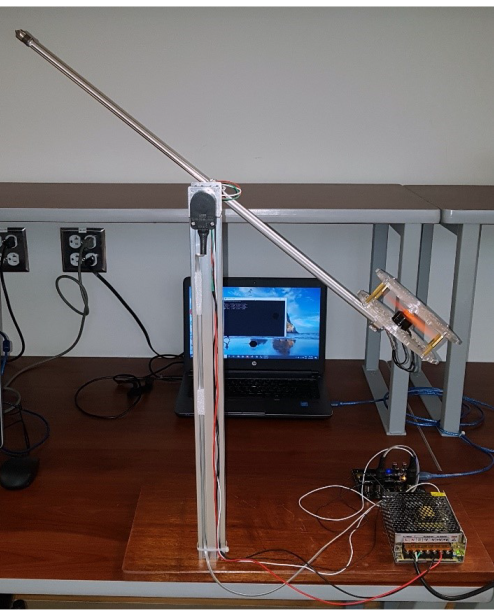
\includegraphics[width=0.3\textwidth]{fig/new/PAMH.png}
    \caption{Planta de laboratorio PAMH \textcolor{SkyBlue}{TesisJorge}.}
    \label{fig:PAMH}
\end{figure}

\begin{figure}[h]
    \centering
    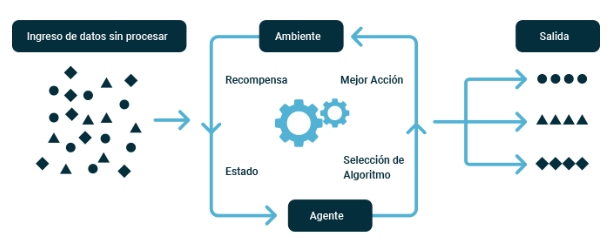
\includegraphics[width=0.6\textwidth]{fig/new/EstructuraAR.png}
    \caption{Modelo de aprendizaje reforzado \textcolor{SkyBlue}{FiguraEstructAR}.}
    \label{fig:EstructuraAR}
\end{figure}

Se realizó la respectiva valoración con una matriz de Pugh que expusiera los puntos a considerar para la elección de la alternativa.

\subsection{Solución 1}

Una red neuronal recurrente (\textit{Recurrent Neural Network}, RNN) presenta su mejor desempeño en el reconocimiento de la voz, donde las secuencias de datos son considerablemente grandes para obtener un entrenamiento eficiente de un modelo, ya que este recorre la trayectoria de los datos en el tiempo, donde cada punto representa un grado de optimización del modelo \textcolor{SkyBlue}{DataScience}.

\subsection{Solución 2} \label{SolucionSeleccionada}

Los métodos de aprendizaje reforzado profundo (\textit{Deep Reinforcement Learning}, DRL) presentan un aumento de la demanda y desarrollo en el área de control, de manera que permiten realizar cálculos complejos y representarlos de manera eficiente en espacios de estados de dimensiones altas, logrando un muy buen desempeño en tareas como el reconocimiento de imágenes \textcolor{SkyBlue}{DataScience}.

\subsection{Solución 3}

Métodos clásicos de aprendizaje reforzado como los cálculos basados en el gradiente o las iteraciones de políticas o valores pueden llegar a representar un camino claro para lograr comportamientos deseados en aplicaciones de control, donde se encuentran diferentes algoritmos que permiten optimizar el entrenamiento de los modelos al aplicar fórmulas específicas para cada método y comportamiento deseado \textcolor{SkyBlue}{DataScience}.


\subsection{Selección de la solución}

Como se observa, cada alternativa corresponde a un modelo de trabajo al aplicar el aprendizaje automático en el control de una planta de laboratorio PAMH, de manera que se considerarán aspectos en los que se evidencia la elección de la solución \ref{SolucionSeleccionada} como la más adecuada para el trabajo en cuestión, esto mediante las valoración en la matriz de Pugh del cuadro \ref{tab:MatrizPugh}.

\begin{table}[h]
\caption{Matriz de Pugh de las opciones de solución.}
\begin{tabular}{lcccc}
\hline
\multicolumn{1}{|c|}{\multirow{2}{*}{\textbf{Criterios}}} &
  \multicolumn{1}{c|}{\multirow{2}{*}{\textbf{Peso}}} &
  \multicolumn{3}{c|}{\textbf{Alternativas}} \\ \cline{3-5} 
\multicolumn{1}{|c|}{} &
  \multicolumn{1}{c|}{} &
  \multicolumn{1}{l|}{\textbf{Solución 1}} &
  \multicolumn{1}{l|}{\textbf{Solución 2}} &
  \multicolumn{1}{l|}{\textbf{Solución 3}} \\ \hline
\multicolumn{1}{|l|}{\begin{tabular}[c]{@{}l@{}}Fiabilidad de control del PAMH\end{tabular}} &
  \multicolumn{1}{c|}{4,5} &
  \multicolumn{1}{c|}{0} &
  \multicolumn{1}{c|}{+1} &
  \multicolumn{1}{c|}{+1} \\ \hline
\multicolumn{1}{|l|}{Costo económico} &
  \multicolumn{1}{c|}{4} &
  \multicolumn{1}{c|}{0} &
  \multicolumn{1}{c|}{+1} &
  \multicolumn{1}{c|}{-1} \\ \hline
\multicolumn{1}{|l|}{Tiempo de desarrollo} &
  \multicolumn{1}{c|}{3,5} &
  \multicolumn{1}{c|}{0} &
  \multicolumn{1}{c|}{+1} &
  \multicolumn{1}{c|}{-1} \\ \hline
\multicolumn{1}{|l|}{Código existente} &
  \multicolumn{1}{c|}{3} &
  \multicolumn{1}{c|}{+1} &
  \multicolumn{1}{c|}{+1} &
  \multicolumn{1}{c|}{+1} \\ \hline
\multicolumn{1}{|l|}{Optimización} &
  \multicolumn{1}{c|}{2,5} &
  \multicolumn{1}{c|}{-1} &
  \multicolumn{1}{c|}{+1} &
  \multicolumn{1}{c|}{0} \\ \hline
\multicolumn{1}{|l|}{Tiempo de entrenamiento} &
  \multicolumn{1}{c|}{2} &
  \multicolumn{1}{c|}{-1} &
  \multicolumn{1}{c|}{+1} &
  \multicolumn{1}{c|}{0} \\ \hline
\multicolumn{1}{|l|}{Datos de entrenamiento} &
  \multicolumn{1}{c|}{1,5} &
  \multicolumn{1}{c|}{0} &
  \multicolumn{1}{c|}{0} &
  \multicolumn{1}{c|}{+1} \\ \hline
\multicolumn{1}{|l|}{Innovación} &
  \multicolumn{1}{c|}{1} &
  \multicolumn{1}{c|}{+1} &
  \multicolumn{1}{c|}{+1} &
  \multicolumn{1}{c|}{+1} \\ \hline
 &
  \multicolumn{1}{l}{} &
  \multicolumn{1}{l}{} &
  \multicolumn{1}{l}{} &
  \multicolumn{1}{l}{} \\ \cline{1-1} \cline{3-5} 
\multicolumn{1}{|l|}{\textbf{Suma general}} &
  \multicolumn{1}{c|}{} &
  \multicolumn{1}{c|}{-0.5} &
  \multicolumn{1}{c|}{20.5} &
  \multicolumn{1}{c|}{2.5} \\ \cline{1-1} \cline{3-5} 
\multicolumn{1}{|l|}{\textbf{Ranking}} &
  \multicolumn{1}{c|}{} &
  \multicolumn{1}{c|}{3"o} &
  \multicolumn{1}{c|}{1"o} &
  \multicolumn{1}{c|}{2"o} \\ \cline{1-1} \cline{3-5} 
\end{tabular}
\label{tab:MatrizPugh}
\end{table}


Con base en la matriz de Pugh desarrollada en el cuadro \ref{tab:MatrizPugh}, se seleccionaron ocho variables que permitieron puntuar los criterios para cada posible solución. 

En primera, se cuenta con la fiabilidad del control del PAMH, eso debido a que algunos métodos no encajan muy bien con el enfoque del proyecto, por lo que es necesario reaccionar en primera instancia con los objetivos que suelen sumarse a cada solución, donde la solución 1 no suele relacionarse con el control de un sistema en específico \textcolor{SkyBlue}{DataScience}.

El costo económico va en función del tiempo de desarrollo, compuesto del entrenamiento y optimización del modelo en cuestión, por lo que el costo computacional y presencial a largos periodos de tiempo es significativo, todo esto frente al tiempo limitado disponible para la elaboración del trabajo final de graduación. 

Cada método presenta características complejas respecto a la implementación de los modelos de aprendizaje automático actuales, por lo que es de vital importancia disponer de referencias bibliográficas que permitan el acceso a códigos de prueba y así, realizar las modificaciones pertinentes, de manera que el constante desarrollo de métodos de aprendizaje automático cumple con este punto.

Dada la teoría y las características de cada solución presentada, la optimización de cada método equivale a diferentes grados de complejidad, donde la solución 1 requiere ajustes adicionales de la estructura para lograrlo, mientras que el caso de los métodos clásicos de RL y DRL permiten un ajuste más cercano a la experiencia y recompensa, en este caso resaltando la solución 2 por su enfoque directo al control de comportamientos \textcolor{SkyBlue}{DataScience}.

Respecto al tiempo de entrenamiento, la estructura secuencial de las RNN castiga especialmente este punto, además de la cantidad de datos de entrenamiento, mientras que el RL mejora este ámbito al aprovechar los recursos computacionales, especialmente el caso del DRL. Es así que los métodos clásicos de RL requieren menor cantidad de datos de entrenamiento pero mayor tiempo de iteración para optimizar, superado fácilmente por el DRL \textcolor{SkyBlue}{DataScience}.

Por último, al tratarse de un área de estudio en auge, constantemente se publican nuevos avances y métodos para cada tipo de modelo de aprendizaje automático, de manera que a nivel general cada solución significa innovación en sus estructuras.

Así y en suma, la solución con valor aceptable se trata de la número 2, donde el caso a utilizar se trata del aprendizaje reforzado profundo (DRL), por sus cualidades más enfocadas al problema en cuestión del proyecto.

En la Figura \ref{fig:Diagbloques} se muestra el diagrama de bloques de la solución propuesta, lo cual permite plantear un primer enfoque de la metodología a desarrollar.

\begin{figure}[!h]
    \centering
    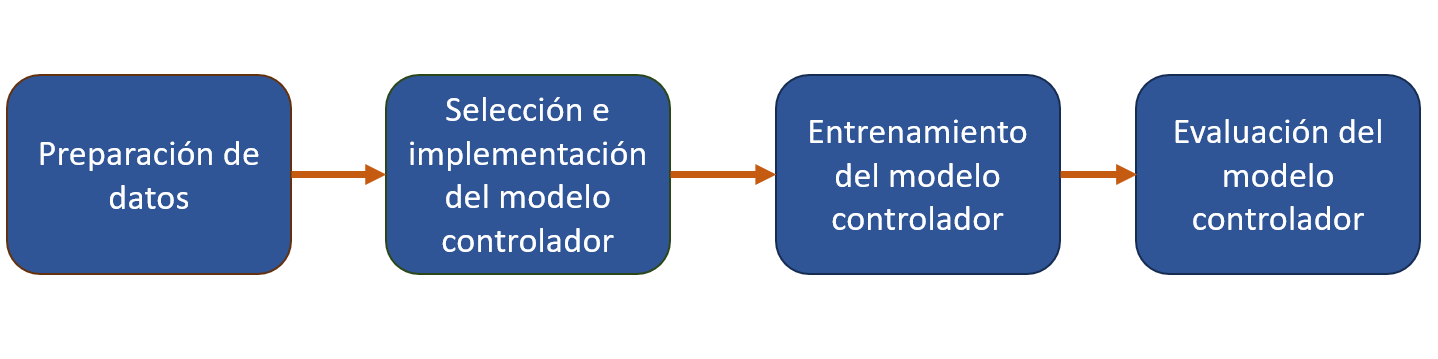
\includegraphics[width=0.7\textwidth]{fig/new/Diagbloques.png}
    \caption{Diagrama de bloques del proceso simplificado de aprendizaje reforzado profundo.}
    \label{fig:Diagbloques}
\end{figure}

\begin{comment}
Bajo dicha modalidad de trabajo se espera el cumplimiento de algunas condiciones necesarias para un correcto entrenamiento y validación del modelo a elaborar, las cuales se muestran en el cuadro \ref{tab:condiciones}
\end{comment}
Bajo dicha modalidad de trabajo se espera el cumplimiento de algunos requisitos necesarios para un correcto entrenamiento y validación del modelo a elaborar, los cuales se muestran en el cuadro \ref{tab:requisitos}

\begin{comment}
\begin{table}[!h]
\caption{Conjunto de condiciones mínimas necesarias para un entrenamiento eficiente del modelo.}
\label{tab:condiciones}
\centering
\begin{tabular}{|c|c|c|}
\hline
\centering\cellcolor{tableheader}\textcolor{white}{\textbf{Parámetro}} & \centering\cellcolor{tableheader}\textcolor{white}{\textbf{Entrenamiento}} & \cellcolor{tableheader}\textcolor{white}{\textbf{Validación y prueba}} \\ \hline
\textit{Conjunto de datos} & 500 episodios          & 100 episodios                \\ \hline
\textit{Duración}          & 3 segundos             & 3 segundos                   \\ \hline
\end{tabular}
\end{table}
\end{comment}

\begin{table}[!h]
\caption{Conjunto de requisitos para la comunicación del controlador mediante DRL.}
\label{tab:requisitos}
\centering
\begin{tabular}{|c|p{11cm}|}
\hline
\centering\cellcolor{tableheader}\textcolor{white}{\textbf{Número}} & {\centering\cellcolor{tableheader}\textcolor{white}{\textbf{Requisito}}} \\ \hline
$1$ & Sistema de captura lee el estado y aplica la acción en tiempo continuo. \\ \hline
$2$ & Sistema de captura de datos capaz de usarse con planta real y planta simulada. \\ \hline
$3$ & Sistema de captura puede acoplarse al controlador con señal de entrada y salida. \\ \hline
\end{tabular}
\end{table}



\section{Objetivo General}

Diseñar un sistema de aprendizaje automático para el control del ángulo de una planta no lineal PAMH.

\textbf{Indicador:} Sistema capaz de alcanzar un error angular inferior al $10\%$ frente a un estímulo constante. 

\subsection{Objetivos específicos}

\begin{enumerate}
    \item Seleccionar un método de aprendizaje reforzado apto para el control no lineal.

\textbf{Indicador:} Métrica de matriz de Pugh sobre métodos preseleccionados de aprendizaje reforzado.

    \item Diseñar la estrategia de captura de datos necesarios para el entrenamiento del modelo de aprendizaje reforzado que controle el modelo imitador del prototipo de laboratorio.

\textbf{Indicador:} Cumplimiento de los requisitos tabulados en el cuadro 2.

    \item Implementar el modelo de aprendizaje reforzado para el control del ángulo y entrenamiento del PAMH.

\textbf{Indicador:} Métrica de recompensa acumulada durante el proceso de entrenamiento y sistema entrenado que logra controlar el ángulo de la planta PAMH emulada.

    \item Evaluar el modelo de aprendizaje automático utilizado.

\textbf{Indicador:} Evaluación de al menos 5 configuraciones distintas de hiperparámetros del modelo seleccionado.


\end{enumerate}


\begin{comment}

%References

@book{ControlModerno,
  author = {Ogata, K.},
  title = {Ingeniería de Control Moderna},
  edition = {5th},
  year = {2010},
  publisher = {Pearson Educación},
  address = {Madrid},
}

@book{Kuo,
    title = {Sistemas de Control Automático},
    author = {Benjamin C. Kuo},
    isbn = {0-13-304759-8},
    year = {2003},
    publisher = {Prentice Hall Hispanoamericana, S.A},
    edition = {7th},
    address = {México}
}

@book{IntroSistemasControl,
  author = {Perez, M. and Perez Hidalgo, A. and Perez Berenguer, E.},
  title = {Introducción a los sistemas de control y modelo matemático para sistemas lineales invariantes en el tiempo},
  year = {2008},
  publisher = {Universidad Nacional de San Juan},
  address = {Argentina},
}

@book{SistemaAlmidon,
  author = {Almidón Elescano, Á. and Julian-Laime, E.},
  title = {Sistemas de Control Automático I - Teoría y problemas aplicativos},
  year = {2018},
  doi = {10.5281/zenodo.2560185},
}

@online{MarketResearch,
    author = "Allied Market Research",
    title = "Artificial Intelligence in Process Control Market by Offering, Technology, and Application: Global Opportunity Analysis and Industry Forecast, 2019-2026",
    url  = "https://www.alliedmarketresearch.com",
    year = "2019"
}

@misc{UniversidadesIA,
  author = {Goncharenko, V.},
  title = {10 Best Universities to Study Artificial Intelligence},
  howpublished = {\url{https://mpost.io/es/10-best-universities-to-study-artificial-intelligence/}},
  year = {2023},
}

@article{MachineLearning,
author = {M. B. Jatana and R. Jain},
year = {2018},
pages = {2319-2325},
title = {A survey on machine learning techniques for educational data mining},
journal = {2018 International Conference on Advances in Computing, Communications and Informatics (ICACCI)},
doi = {10.1109/ICACCI.2018.8554968}
}

@online{SIPLab,
    author = "SIPLab",
    title = "¡Bienvenidos al sitio web del SIP-Lab!",
    url  = "http://www.ie.tec.ac.cr/palvarado/pmwiki/index.php/Main/HomePage",
    year = "2020"
}

@book{AprendRefor,
    title = {Reinforcement Learning: An Introduction},
    author = {Richard S. Sutton and Andrew G. Barto},
    year = {2018},
    publisher = {MIT Press},
    address = {England}
}

@book{DataScience,
    title = {Data-Driven Science and Engineering},
    author = {Steven L. Brunton and J. Nathan Kutz},
    year = {2021},
    publisher = {Cambridge University Press},
}

@book{Control,
  title={Control Systems Engineering},
  author={Nise, Norman S},
  year={2011},
  publisher={John Wiley \& Sons},
}

@misc{BBVA,
  author = {BBVA: Communications},
  title = {Machine learning: What is it and how does it work?},
  howpublished = {BBVA},
  year = {2019},
  url = {https://www.bbva.com/en/innovation/machine-learning-what-is-it-and-how-does-it-work/}
}

@misc{VideoIA,
  author = {Scouting y Promoción Uniandes},
  title = {¿Cómo Aplicamos la Inteligencia Artificial en Ingeniería Eléctrica y Electrónica?},
  howpublished = {YouTube},
  year = {2021},
  url = {https://www.youtube.com/watch?v=tlm5s5KGKqg}
}

@mastersthesis{TesisJorge,
  author  = "Jorge Andrés Brenes Alfaro",
  title   = "Diseño e implementación de un sistema que simule el comportamiento dinámico de una planta prototipo de control automático utilizando redes neuronales artificiales",
  school  = "Instituto Tecnológico de Costa Rica",
  year    = "2022",
  address = "Costa Rica",
}

@misc{PAMHinfo,
  author = {Soto Cárdenas, R.},
  title = {PROYECTO CORTO. Tema: Identificación y control del péndulo amortiguado a hélice (PAMH).},
  howpublished = {DOCPLAYER},
  year = {2021},
  url = {https://docplayer.es/209372927-Proyecto-corto-tema-identificacion-y-control-del-pendulo-amortiguado-a-helice-pamh.html}
}

@misc{FiguraEstructAR,
  title={Aprendizaje por Refuerzo},
  author={Nancy Velazquez},
  year={2021},
  howpublished={\url{https://trustnet.com.mx/aprendizaje-por-refuerzo/}}
}

\end{comment}

















\section{*************************************************}


En la \nt{introducción} deben quedar completamente claros los siguientes
aspectos, cuyo significado depende del tipo concreto de tesis:

\begin{compactitem}
\item Contexto
\item Antecedentes
\item Problema concreto
\item Esbozo de solución
\item Objetivos y estructura
\end{compactitem}

Una buena introducción debe lograr que el lector tenga interés de leer el resto
del tesis.

Es recomendable dividir la tesis en secciones, nombradas cada una de acuerdo a
su contenido. \textbf{Jamás} utilice los nombres de la guía como
``\emph{Problema existente e importancia de su solución}'', sino algo como ``La
deforestación en Costa Rica'' o lo que se adecúe a su problema en particular.

Recuerde que en español solo la primera letra del título va en mayúscula
(exceptuando nombres propios, por supuesto).
%
Algunos recursos adicionales a esta guía los encuentra en \cite{AlvaradoWeb}.


\section{El cambio climático y la electrónica}
\label{sec:contexto}

El contexto corresponde al entorno donde se desarrolla el proyecto de
tesis, que puede ser el área general de aplicación, un dominio de
problemas, etc.

De nuevo, no use un título genérico como ``Contexto'', sino algo
asociado directamente a su trabajo.


\section{Antecedentes}

Si su proyecto se circunscribe en otro proyecto mayor, en el que han
participado otros estudiantes de grado y postgrados, y ya existen
tesis o artículos publicados, en esta sección se hace una breve reseña
de esos trabajos previos, con el objetivo de contextualizar en dónde
calza concretamente el trabajo actual dentro de ese otro proyecto
mayor.  Por ejemplo, Fulano en~\cite{Fulano21} exploró si un diodo
puede funcionar como fuente de energía infinita, hipótesis que no
logró comprobar.

En proyectos relativamente aislados, no es necesaria esta sección.

Dependiendo de cada trabajo concreto, esta sección puede desplazarse a
otro lugar dentro de la introducción donde tenga más sentido, pero
usualmente se encuentra aquí justo antes de presentar el problema
técnico concreto tratado en su proyecto.

\section{La disipación de energía en el reactor 42}

En esta sección usted debe exponer su problema concreto.  Debe enlazar
el contexto general, expuesto en las secciones anteriores, con el
problema concreto que este trabajo resuelve.

Al final de esta sección, el problema concreto se sintetiza usualmente
en una frase de planteamiento del problema de ingeniería o pregunta
generadora de la investigación de ingeniería. Esta frase o pregunta
debería ser una consecuencia a la que se llega después de realizar el
desarrollo del contexto.  Si el problema es de caracter científico,
aquí puede plantearse la hipótesis de la investigación científica.

Del planteamiento del problema se deriva cuál es el objetivo del
trabajo en particular, que a su vez debe conducir al lector de forma
natural al esbozo de la solución del problema a tratar en este
informe.

\section{Sistema de almacenamiento energético}

Después de las secciones anteriores ya ha guiado al lector hasta este
punto en donde solo resta presentar una propuesta general de solución
del problema técnico concreto.

Para aclarar la solución se hace uso de un diagrama de bloques (ver
\figref{fig:diagbloques}) o diagrama de flujo general, es decir,
desde un nivel de abstracción muy alto, donde no sea necesario entrar
en detalles técnicos, porque aun no han sido expuestos.

\begin{figure}[htb]

  %% Este es un ejemplo de figura TIKZ incrustada directamente
  %% en el la figura, pero es muchísimo más recomendable poner este
  %% código, tal y como se explica en el siguiente capítulo, en un archivo
  %% aparte.  Como archivo aparte se puede compilar la figura una sola vez
  %% para que quede disponible en el directorio fig/.  Eso es más rápido de
  %% compilar posteriormente.
  %%
  %%
  %% Se coloca este ejemplo aquí porque muchas personas están usando
  %% Overleaf, y allí puede tener sentido tener las figuras
  %% directamente en el código del informe, aunque esto tardará más en
  %% compilar e incluso puede llevar a Overleaf a pasarse del tiempo
  %% disponible.
  
  \centering
  \tikzstyle{block} = [draw, rectangle, inner sep=6pt]
  \begin{tikzpicture}[>=latex,auto,node distance=2cm]
    \node [block](system) {Sistema};
    \node [coordinate, left=of system] (infork) {};
    \node [coordinate, left=of infork] (input) {};
    \node [coordinate, right=of system] (outfork) {};
    \node [coordinate, right=of outfork] (output) {};
    \node [block, below=of system] (storage) {Almacenamiento};

    \node [block, dashed, fill=gray, anchor=center, text width=7cm, align=center] at ($(system)!.5!(storage)$) {Conversión};

    % Connect nodes
    \draw [->] (input) -- node {$E_i$} (system);
    \draw [->] (system) -- node {$E_o$} (output);
    \draw [->] (storage) -| (outfork);
    \draw [->] (infork) |- (storage);
  \end{tikzpicture}
  \caption[Diagrama de bloques.]{Diagrama de bloques del sistema
    propuesto de almacenamiento energético, como ejemplo de código
    TikZ insertado directamente en el texto (ver archivo
    \code{intro.tex}, línea \number\inputlineno).}
  \label{fig:diagbloques}
\end{figure}

Nótese que un diagrama de bloques es distinto a un diagrama de etapas.
En general para este informe se prefiere el diagrama de bloques, pues
el diagrama de etapas tiene una connotación de documentación de
bitácora, que no es el objetivo de este informe.  Aquí se debe
explicar cómo reproducir los resultados a que finalmente se llegó, en
vez de explicar el proceso circunstancial y particular que usted
siguió para hacerlo; es decir, el proceso que usted siguió
posiblemente requirió pruebas fallidas y otras exploraciones que no
viene al caso explicar aquí (pero que usted sí documenta en su
bitácora, que es otro documento aparte), sino que aquí lleva al lector
por la ruta de exito directamente.

Usualmente este diagrama y su breve explicación dictan cuál será la
estructura del resto del documento, pues usted en el
\capref{ch:marco} deberá explicar los fundamentos teóricos que
cada bloque en esa solución requiere, y en el
\capref{ch:solucion} presentará una versión con mayor detalle de
esa solución, en donde ya considera lo expuesto en el marco teórico.



\section{Objetivos y estructura del documento}

\index{objetivos}
Esta plantilla LaTeX tiene como objetivo simplificar la construcción del
documento de tesis, presentando ejemplo de figuras y \tablas, así como otorgar
una plataforma de compilación en GNU/Linux que simplifique la administración de
todo el documento.

La última sección de la introducción usualmente sí tiene un título estandar que
es ``Objetivos y estructura del documento'', donde se presentan \emph{en prosa}
los objetivos general y específicos que ha tenido el proyecto de tesis,
así como la estructura de la tesis (por ejemplo, ``en el siguiente capítulo se
esbozan los fundamentos teóricos necesarios para explicar en el
\capref{ch:solucion} la propuesta realizada$\ldots$''

%%% Local Variables: 
%%% mode: latex
%%% TeX-master: "main"
%%% End: 
